\documentclass[12pt,halfparskip]{scrartcl}

\newcommand{\dokumenttitel}{Erfahrungsberichte}
\usepackage{../bodesuri}


\begin{document}

\title{\dokumenttitel}
\titlehead{
	\centering
	
\includegraphics[width=0.5 \textwidth, clip, trim = 0 7cm 0 0]{design/externes_design/bodesuri_plakat}
	\vspace{2cm}
}
\author{Danilo~Couto, Philippe~Eberli, \\ Pascal~Hobus, Reto~Schüttel, Robin~Stocker}
\maketitle
\newpage

\pagenumbering{roman}

\tableofcontents
\thispagestyle{plain}
\newpage

\pagenumbering{arabic}

\markright{Bodesuri -- \dokumenttitel}


\section{Erfahrungsbericht von Edgar Danilo Couto}

In einem solch grossen Entwicklungs-Projekt war ich bis jetzt noch nicht involviert gewesen. Wie auch schon in anderen Projekten habe ich in diesem wieder viele neue Erfahrungen gesammelt. Die wichtigste Erkenntnis war, wie wichtig die Kommunikation zwischen den einzelnen Projektmitgliedern ist und wie gross der Overhead bei einem grossen Team sein kann. Die Kommunikation zwischen den einzelnen Projektmitgliedern haben wir mittels Sitzungen, E-Mails, Chatclient und IRC sehr gut gemeistert.

Der Anreiz am Projekt war es ein PC-Spiel zu entwickeln mit einem interaktiven GUI. Es war eine neue Herausforderung ein solches GUI zu implementieren und seit einer Ewigkeit auch ein grosser Wunsch meinerseits. Am Anfang sah es danach aus, als ob Swing nicht dafür geschaffen sei und ich hatte es mit Java 2d versucht. Die Möglichkeit von geometrischen Objekten zu gestalten ist in Java 2d hervorragend gelöst. Doch das Ansprechen der einzelnen Objekte im GUI war zu kompliziert. Wir haben uns dann wieder für Swing entschieden. Ich war aber noch sehr skeptisch, aber es erwies sich als eine sehr gute Entscheidung. Der Code sah um einiges einfacher aus und man konnte einfach mittels Observer die Objekte ansprechen und deren neues Aussehen mitteilen. 

Sehr grossen Spass hatte ich auch beim entwerfen der Designs im Photoshop. Ich hatte nicht gedacht, dass es Möglich sei, das komplette Design in Swing zu implementieren, so dass es dem Original Design entspricht. Und mit grossem Erstaunen ist uns auch dies geglückt. Let’s Swing. 

Als neue Technologie im GUI habe ich mich mit XML befasst. Das XML wurde für das Layout verwendet. Jede einzelne Grafik ist mittels Koordinaten auf dem Spielbrett positioniert worden. Das GUI ist so konzipiert, dass man in einem weiteren Schritt ein neues Design entwerfen kann und damit spielen, ohne jeglichen Code umzuschreiben.

Ich habe mich gegen den Schluss auch noch um die Website gekümmert, spricht mit dem Wiki. Ich hatte einige Bedenken, dass man damit eine ansprechende Website erstellen kann. Jetzt sehe ich das völlig anders. Für Dokumentationen jeglicher Art ist das Wiki als Framework die richtige Entscheidung. Das barrierenfreie Design ermöglicht einem durch einfache CSS-Erweiterungen eine anspruchsvolle Website zu entwerfen. In den weiteren Projekten werde ich auf jeden Fall wieder auf das Wiki zurückgreifen.

Als Dokumentation haben wir \LaTeX{} verwendet was für mich ganz neu war. Bis jetzt hatte ich nur Word als Dokumentationswerkzeug verwendet gehabt, welches aber für eine grössere Gruppe nicht geeignet ist. Durch SVN und \LaTeX{} konnten alle Projektmitglieder zur selben Zeit am selben Dokument arbeiten, was sehr gut funktioniert hat. Doch die Möglichkeit der Gestaltung des Dokuments ist beschränkt, was ich persönlich sehr schade finde. In den kommenden Projekten werde ich wieder mit Word die Dokumente erstellen.

Zusammenfassend kann ich dazu sagen, dass das Projekt sehr lehrreich war und trotz der grossen Projektgruppe uns alles sehr gut gelungen ist. Wir hatten eine sehr schöne und amüsante Zeit zusammen, obwohl es mit sehr viel Arbeit verbunden war. Ich möchte mich auf diesem Weg noch bei allen Projektmitgliedern und Helfern für den Einsatz herzlich bedanken.


\section{Erfahrungsbericht von Pascal Hobus}

Als wir ganz am Anfang eine Arbeit suchten, die zu fünft gut umsetzbar und auch noch interessant sein soll, war ich noch etwas skeptisch und wusste nicht so recht was denn nun genau geeignet wäre. Als wir dann auf die Idee kamen das Dog-Spiel auf den Computer zu bringen war das für mich gleich ein grosser Motivationsschub, da ich das Spiel regelmässig mit meinen Freunden zuhause spiele und sehr spannend finde. Nachdem wir das Spiel auch einige Male unter uns gespielt hatten und bei allen die gleiche Motivation erkennbar war machte es auch gleich doppelt Spass, da alle immer an einem Strang zogen.

Am Ende der "<Elaboration"> und zu Beginn der "<Construction 1"> Phase habe ich mich sehr stark um die Architektur des Systems gekümmert. Das Modellieren der Architektur hat mir sehr gefallen, da man schnell auf Schwachstellen und zyklische Abhängikeiten gestossen ist, die man flicken konnte und so die Qualität der Software markant verbessern konnte. Je weiter die Implementierung jedoch voranschritt, desto mehr und desto grössere Refactorings gab es. Es zeigte sich dann, dass man im UML-Tool das Modell mit dem Sourcecode hätte verlinken müssen, damit diese Refactorings erkannt worden wären. Dies war auch ein Grund dafür, warum ich dann nicht mehr in so kurzen Zeitintervallen ein Codereverse durchgeführt habe. Mit der Einführung des Tools Structure 101 hat Reto jedoch eine super Alternative gefunden, um die Package- und Klassenhierarchien zu durchforsten und auf Designfehler zu untersuchen.

Was mich etwas gestört hat war, dass ich nicht immer programmieren konnte. Ich hatte oft Lust jetzt "<endlich"> etwas in Java zu implementieren, musste dann aber feststellen dass schon an allen Baustellen gebaut wurde und es keinen Sinn machte, zu zweit den selben Code zu bearbeiten. Und eine neue Baustelle für ein niedriger priorisiertes Arbeitspaket zu erstellen erschien mir dann auch nicht korrekt. Vor allem in den Phasen "<Construction 2"> und "<Construction 3"> gab es dann aber genug Arbeit um auch interessante Sachen zu implementieren (zum Beispiel Teile des Controllers, die Feldauswahl, das VerbindenView und die Lobby oder die Steuerung der Partnerfiguren).

Mit der Dokumentation in \LaTeX{} hatte ich Anfangs eher mühe. Ich finde das Prinzip einer einfachen Textverarbeitung die mit Subversion verwaltbar ist sehr gut. Wir hatten keine Probleme zu fünft am gleichen Dokument zu schreiben. Sobald ich jedoch meine Gedanken zu Papier bringen wollte, musste ich mich stark mit der Syntax (nur am Anfang) und Formatierungsproblemen auseinandersetzen. Ein WYSIWIG Editor ist für mich an dieser Stelle sehr viel effizienter, da ich mich auf das Wesentliche -- die Dokumentierung -- konzentrieren kann. Für eine Studienarbeit sehe ich \LaTeX{} nicht als geeignetes Instrument, da ich damit einfach zu ineffizient dokumentieren kann. Mein Wunschwerkzeug wäre ein guter WYSIWYG-Editor, der \LaTeX{} generiert.

Die Arbeit mit meinen Kollegen im Team fand ich super. Wir konnten gegenseitige Kritik stets äussern und profitierten meines Erachtens stark von den Stärken der anderen. So bin ich zwar noch nicht zum Konsolen-Freund mutiert, denke aber, dass ich in Zukunft möglichst alle repetitiven Arbeiten zum Beispiel mit einem Ruby-Skript lösen sollte. Was ich persönlich in unserem Projekt super fand, ist die gesamte Infrastruktur und Entwicklerwerkzeuge die wir genutzt haben (Trac, CruiseControl, usw.). Die ganze Thematik der Zeiterfassung war eher ein mühsames Anliegen, da wir einfach kein geeignetes Tool fanden und die Excel-Vorlage auch einige Schwachstellen aufwies.
			
Abschliessend kann ich sagen, dass ich mit dem Projekt sehr zufrieden bin und auch zukünftig noch am Spiel weiterentwickeln möchte. Ich würde vor allem noch gerne die Auswahl der Partnerschaft und einen intelligenten Bot hinzufügen. Ich habe den Eindruck, dass dieses Projekt eine sehr gute Vorbereitung auf die Studienarbeit im kommenden Herbst war.

\section{Erfahrungsbericht von Philippe Eberli}

Nachdem wir im Fach Userinterfaces1 bereits ein mini Projekt durchgezogen hatten, dass mich bloss mässig begeistert hatte, freute ich mich nicht besonders auf dieses Projekt. Als jedoch die Idee aufkam Dog umzusetzen stieg meine Begeisterung sprunghaft, da ich dieses Spiel sehr gerne spiele.

Der Projektbeginn gestaltete sich etwas schwierig, denn es galt die Zeiteinteilung für das gesamte Projekt zu machen. Die Schwierigkeit dabei war zu planen, welches Packet wie lange dauern würde. Ein weiterer Aufwand, war der Wechsel unserer Zeiterfassung nach dotProject und wieder zurück ins Excel, was uns Zeit und Nerven kostete. Die Zeitplanungproblematik sollte uns jedoch das ganze Projekt durch begleiten. Einerseits beim Planen der Dauer von Aufgaben, andererseits beim Zuteilen neu auftauchender Aufgaben in existierende Pakete.

Eine sehr interessante Erfahrung war die Software Entwicklung in einem doch schon etwas grösseren Team. Nicht immer hatte es genügend Programmierarbeiten für alle. Ausserdem kennt nicht jeder von uns alle Bereiche unseres Spiels gleich gut. Einige Tools haben uns sehr geholfen die Übersicht zu behalten. Cruisecontrol zwang uns, durch das automatische Testen, nur funktionierenden Code ins Repository zu laden, dank Trac's RSS-Feed hatten alle von uns die Übersicht wer was macht und mit Trac's Wiki konnten wir schnell und einfach Texte schreiben und allen zur Verfügung stellen(z.B. Sitzungsprotokolle). Die Übersicht über den Code auf Designebene zu behalten, half uns Structure 101.

Eine Überraschung war die Dauer der Sitzungen. Jede Woche sassen wir eine bis zwei Stunden zusammen und planten die nächste Woche. Beim Auswerten der Zeiterfassung bemerkten wir, dass ein grosser Teil unserer Zeit in den Sitzungen verbraucht wurde. Ein Umstand der sich durch die fünffache Verrechnung erklären lässt. Es ist schwierig zu sagen ob sich eine Einsparung hier gelohnt hätte, da wir an den Sitzungen wichtige Punkte diskutierten. Eine Hilfe wäre vielleicht eine bessere Planung der Sitzungen gewesen.

Eine weitere interessante Erfahrung war es, keinen Projektleiter zu haben. Es kann sein, dass gewisse Entscheide komplizierter zu Fällen waren oder länger dauerten, da wir zuerst alle Projektmitglieder fragen wollten. Die Vorteilen waren, dass niemand die Verantwortung für das Projekt übernehmen musste und jeder Punkt diskutiert wurde, sich alle eine Meinung bilden konnten und wir am Schluss immer zu einem Konsens kommen konnten. Entweder in einem Kompromiss oder durch Abstimmen.

Die Zusammenarbeit empfand ich als sehr gut. Jeder in unserem Team hat individuelle Stärken, die er einbringen konnte. Neben (während?) der Arbeit verbrachten wir einige unterhaltsame Stunden und hatten viel zu Lachen. Nachdem das Projekt nun zu Ende ist, werden wir sicher noch einige Zeit an Bodesuri weiterentwickeln. Wir haben noch viele Ideen und ich freue mich darauf!

\section{Erfahrungsbericht von Reto Schüttel}

Ein solch grosses Projekt mithilfe von fünf Personen langsam aber stetig entstehen zu entstehen war eine ganz neue Erfahrung für mich. Die relativ grosse Gruppe war bestimmt ein Faktor der nicht immer zu unseren Gusten war. Die Zeit, die die Team-Meetings und sonstige Koordinationen auffrassen, war meines Erachtens imens. Es ist aber nicht so, dass ich usnere Sitzungen als unproduktiv oder ineffizient empfunden habe, aber bei fünf Personen scheint einfach ein viel grösserer Kommunikationsaufwand notwendig zu sein.

Sehr gut gefallen hat mir die Entwicklungsumgebung die wir im Laufe der Zeit aufgebaut haben. Seit etwa Woche 5 oder 6 war eigentlich fast immer einen funktionsfähiges Produkt vom Build-Server erhältlich, seit etwa zwei Wochen ist dieses auch immer auf der Homepage verlinkt und somit quasi "<veröffentlicht">.  Ähnliche wiederholende Aufgaben, zum Beispiel das generieren des Test-Coverage Reportes oder der Dokumenten TODO Liste waren ebenfalls in diesen Prozess eingebunden und standen uns quasi nach commit fast sofort zur Verfügung. Beim nächsten Projekt würde ich vermutlich sgoar noch mehr Zeit von Anfang an in eine solche Infrastruktur investieren. Zum Beispiel ging die Anzahl der defekten Builds massiv zurück als wir begannen, bei fehlgeschlagenen Builds, Mails zu versenden. Eine anderes Thema war die Erstellung von Statistiken, ich musste dieserückwirkend generieren was relativ mühsam war. Zwar ging dies dank svn und dem Scripting Support von Structure 101 recht gut, aber ich denke nächstes Projekt werd ich dies von Anfang an so einrichten und die Statistik vor zu generieren lassen.

Während ich in vielen Bereichen positive Erfahrungen mit den Methoden und Tools gemacht habe und diese auch in ähnlicher Form in zukünftigen Projekten weiterverwenden werde, sticht doch das Thema Zeiterfassung negativ heraus. In der von uns verwendeten Form war die Zeiterfassung und Planung nicht nur aufwändig sondern meiner Meinung nach auch ziemlich sinnlos. Wie sollen wir in der Inception/Elaboration Phase wissen wie lange die Implmentation des Siebnerzuges geht? Bei der konkreten Planung des Features gab es zudem mehrere Varianten mit unterschiedlichem Zeitaufwand. Ich verstehe dass der Kunde von Anfang an eine ungefähre Zeitabschätzung benötigt, aber ich würde in meinem nächsten Projekt die Detailzeitplanung (Soll Stunden pro Paket) erst wirklich in der jeweiligen Phase machen. Vorher müsste man unter Umständen einfach einem ganzen Themenbereich (z.B. Regelsystem) einen Total-Stunden Wert zuordnen der anschliessend für die Implementation der einzelnen Features verbucht werden könnte. Geht in einem Bereich die Zeit aus muss auf die Implementaiton weiterer Features verzichtet werden. So oder so, die Zeitplaung und Erfassung war meines Erachtens unbefriedigend und frustrierend.

Mir hat das Team und das Projekt im allgemeinen viel Spass gemacht. Man konnte viel lernen und ich denke das Endprodukt kann sich sehen lassen. Ich möchte meinen Teammitgliedern für die tolle Zusammenarbeit danken, gerne wieder!

\section{Erfahrungsbericht von Robin Stocker}

\section{Team-Erfahrungsbericht}
In unserem Team haben wir die Erfahrung gemacht, dass die Bestimmung eines Projektleiters nicht notwendig war. Entscheidungen haben wir demokratisch gefällt und auch akzeptiert, wenn sie nicht unbedingt der eigenen Meinung entsprach. Was für uns eindrücklich erschien, war die benötigte Zeit die wir in Sitzungen investiert haben. Es erschien uns dann aber logisch, da eine Sitzung ja aber immer für jedes Teammitglied ins Gewicht fiel.

Was bei dem Diagramm der Zeitabweichung gut ersichtlich ist, ist der Umstand, dass wir vor einer Abgabe immer ziemlich viel mehr Zeit investieren mussten als geplant. Ein extremes Beispiel war die "<Designabgabe">. Dort sieht man einen deutlichen Ausschlag. Auch gegen Projektende mussten wir mehr Zeit investieren als vorangeschlagen war. Da aber keiner von uns einfach Features streichen wollte war es für alle klar, dass wir die geforderten Features auf jeden Fall implementieren würden. Wir hatten alle Spass am Projekt und deshalb war es für keinen von uns ein Problem. Unter dem Strich haben wir jedoch schon etwas mehr Zeit benötigt als geplant.

\begin{figure}[h]
	\centering
	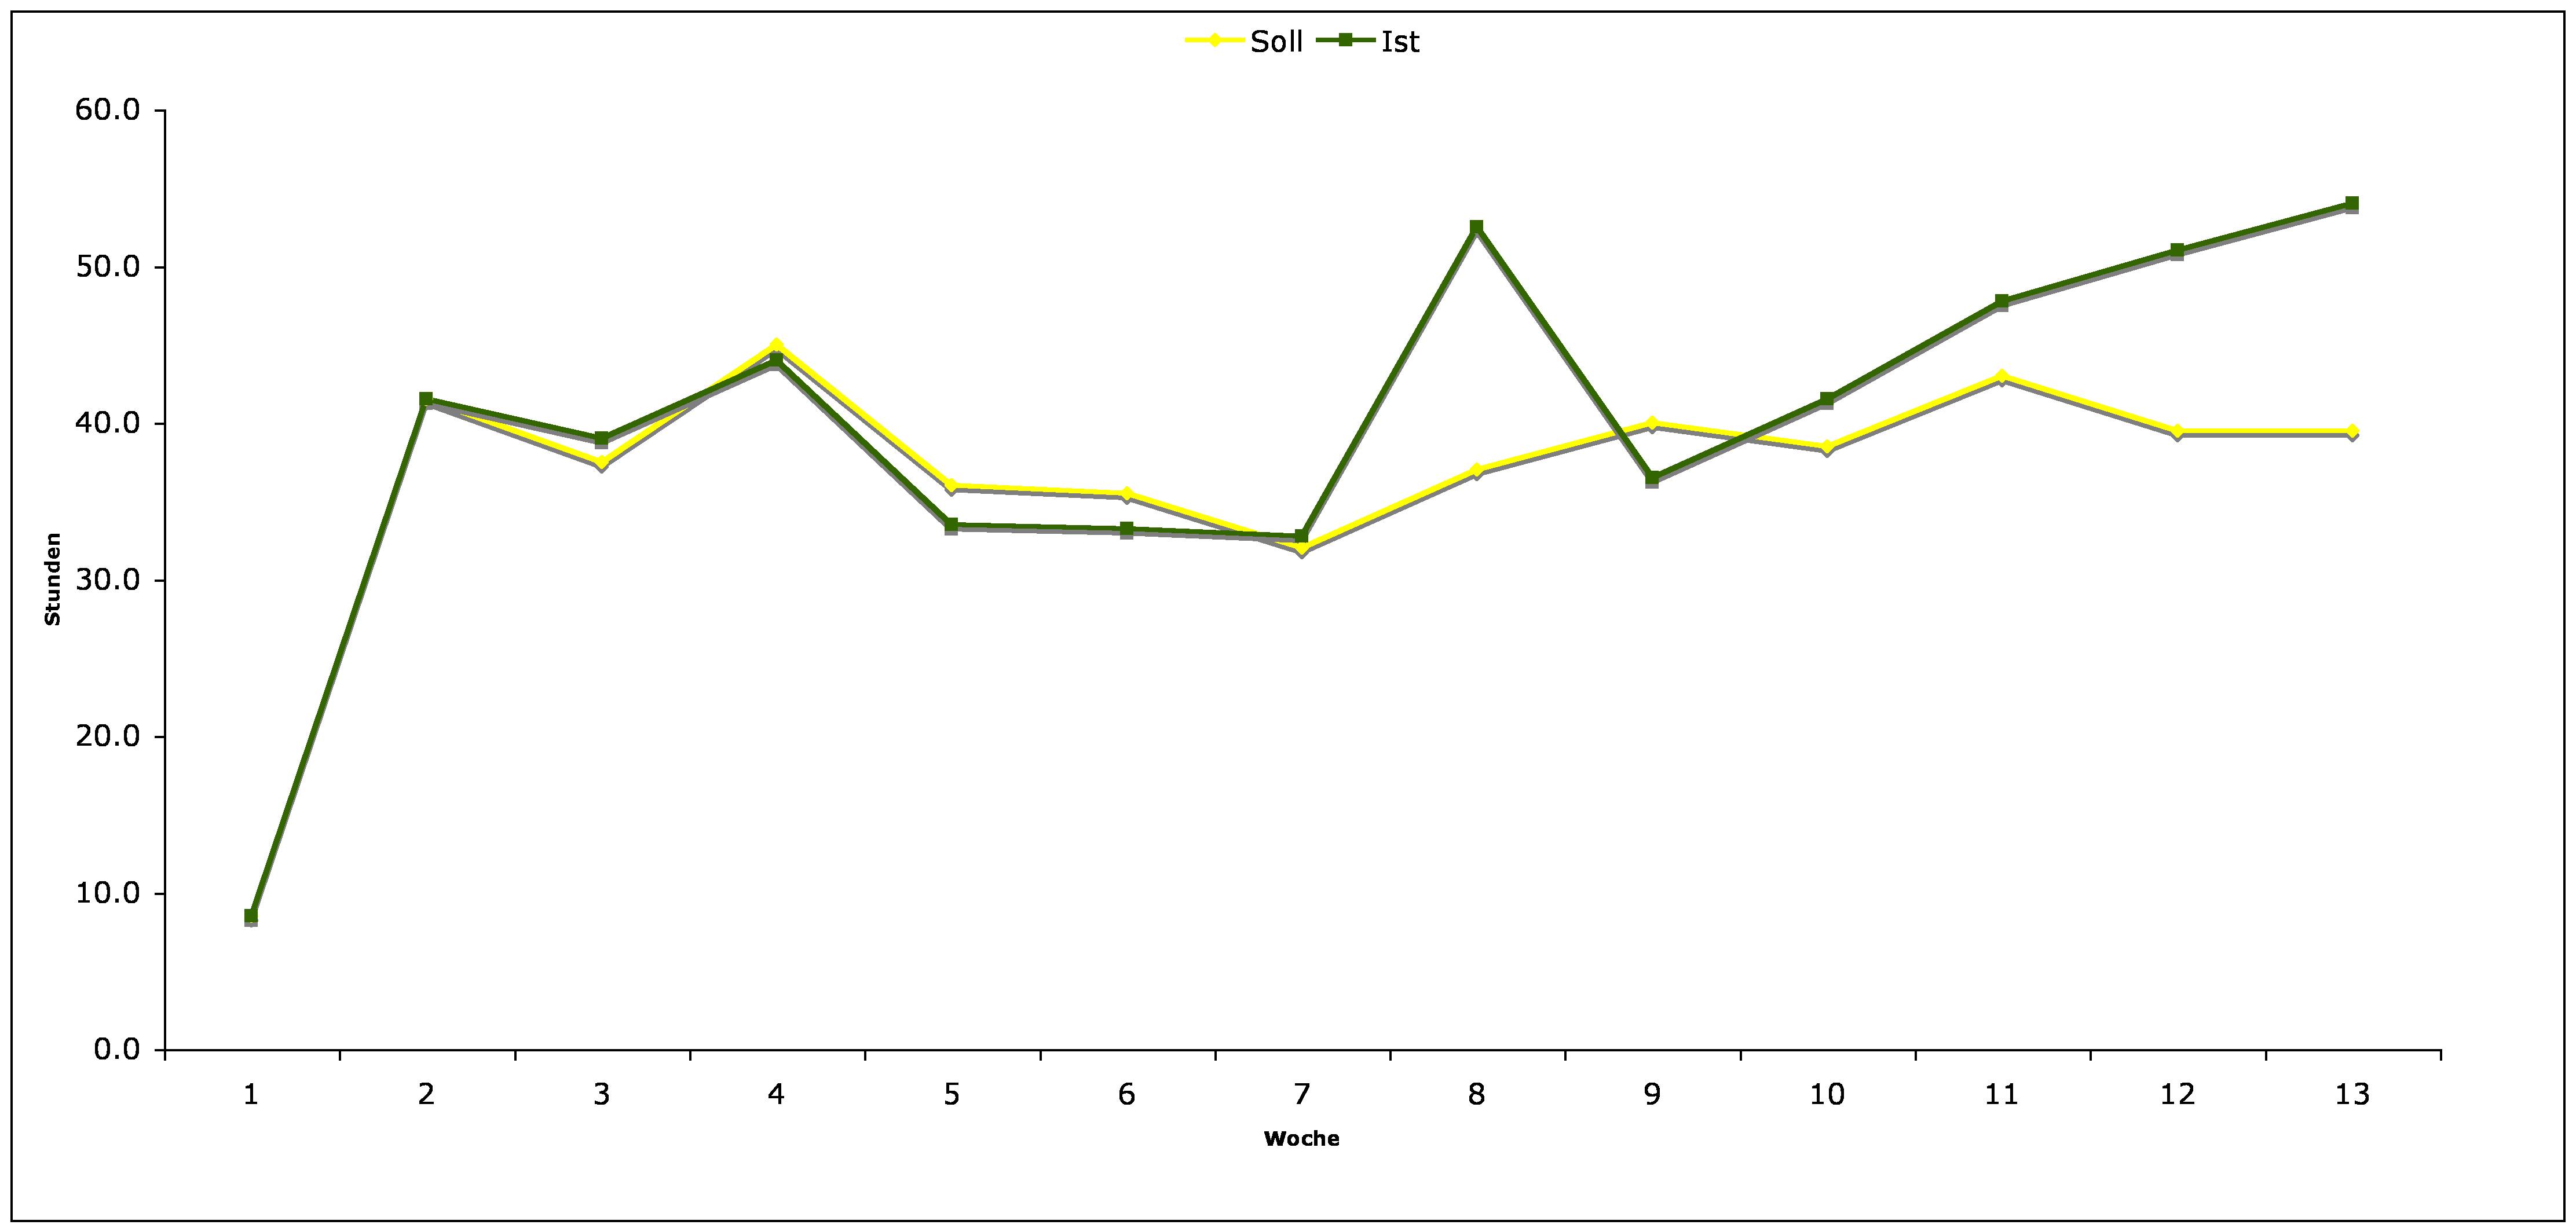
\includegraphics[width=0.8 \textwidth]{zeitabweichung}
	\caption{Zeitabweichung bei der Planung}
	\label{fig:zeitabweichung}
\end{figure}

\begin{figure}[h]
	\centering
	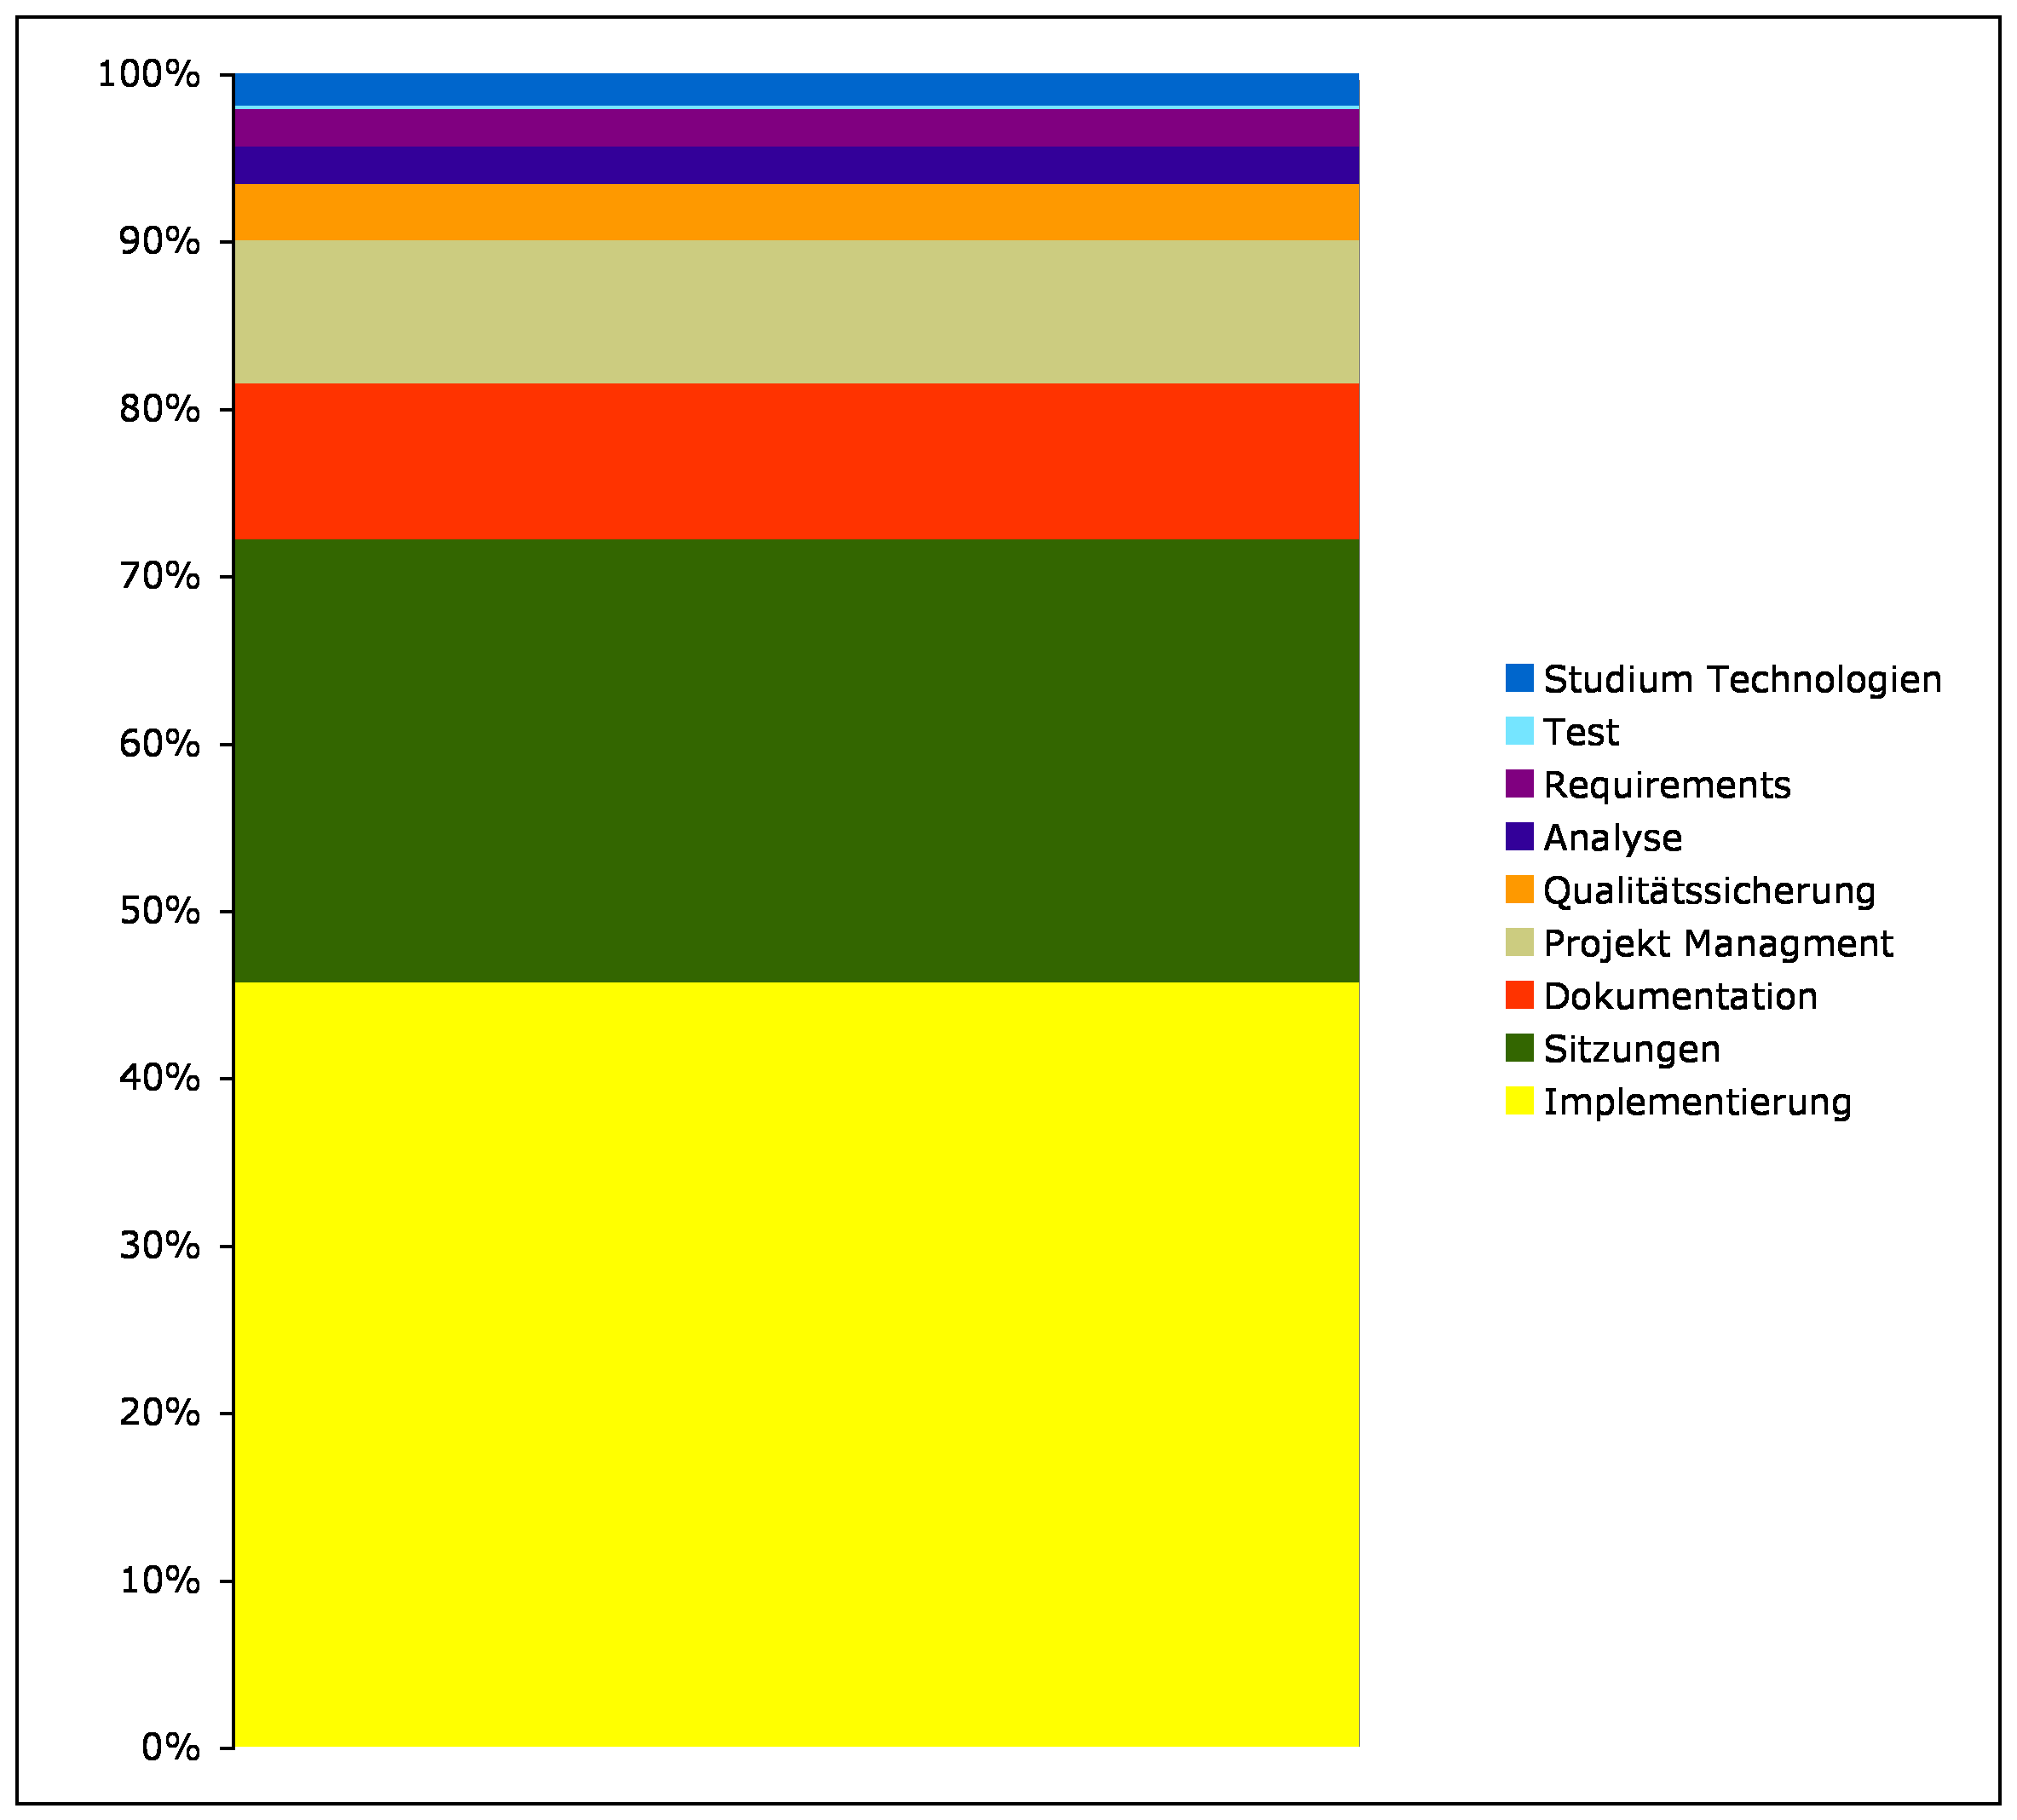
\includegraphics[width=0.8 \textwidth]{zeitbeachspruchung_arbeiten}
	\caption{Zeitbeanspruchung verschiedener Arbeiten}
	\label{fig:zeitbeachspruchung_arbeiten}
\end{figure}

\section{Statistiken}
\subsection{Testabdeckung aller Packages}

% TODO: Robin: kann man Bilder Seiten irgendwie mit clearpage und H und clearpage querformat machen? Das geht doch sicher? (-reto)
Unsere JUnit-Tests erreichen über das gesamte Projekt gesehen eine relativ hohe Abdeckung von 79 Prozent. Dabei muss noch berücksichtigt werden, dass das UI nicht durch JUnit-Tests getestet wird. Durch die Zuhilfenahme des Bots stieg die Abdeckung auch noch um ein grosses Stück, da dieser beinahe alle Teile des Codes benötigt. Wenn dann ein Spiel mit Bots zu Ende gespielt wurde, so verläuft der Test erfolgreich.

Markant ist, dass die Problem-Domain eine sehr hohe Testabdeckung aufweist und auch während des ganzen Projektes aufgewiesen hat. Diese konnte so immer als sehr stabile Grundlage für die Entwicklungen dienen.
\begin{figure}[h]
	\centering
	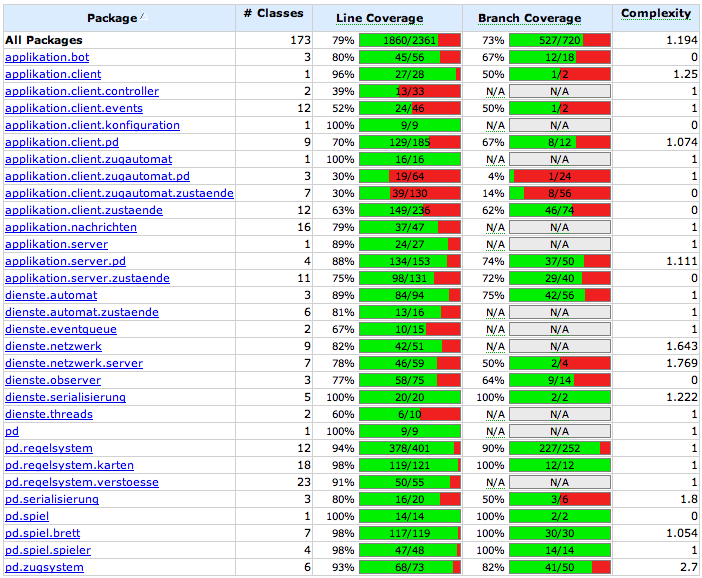
\includegraphics[width=0.8 \textwidth]{test_abdeckung_gesamt}
	\caption{Testabdeckung aller Packages}
	\label{fig:test_abdeckung_gesamt}
\end{figure}
\begin{figure}[h]
	\centering
	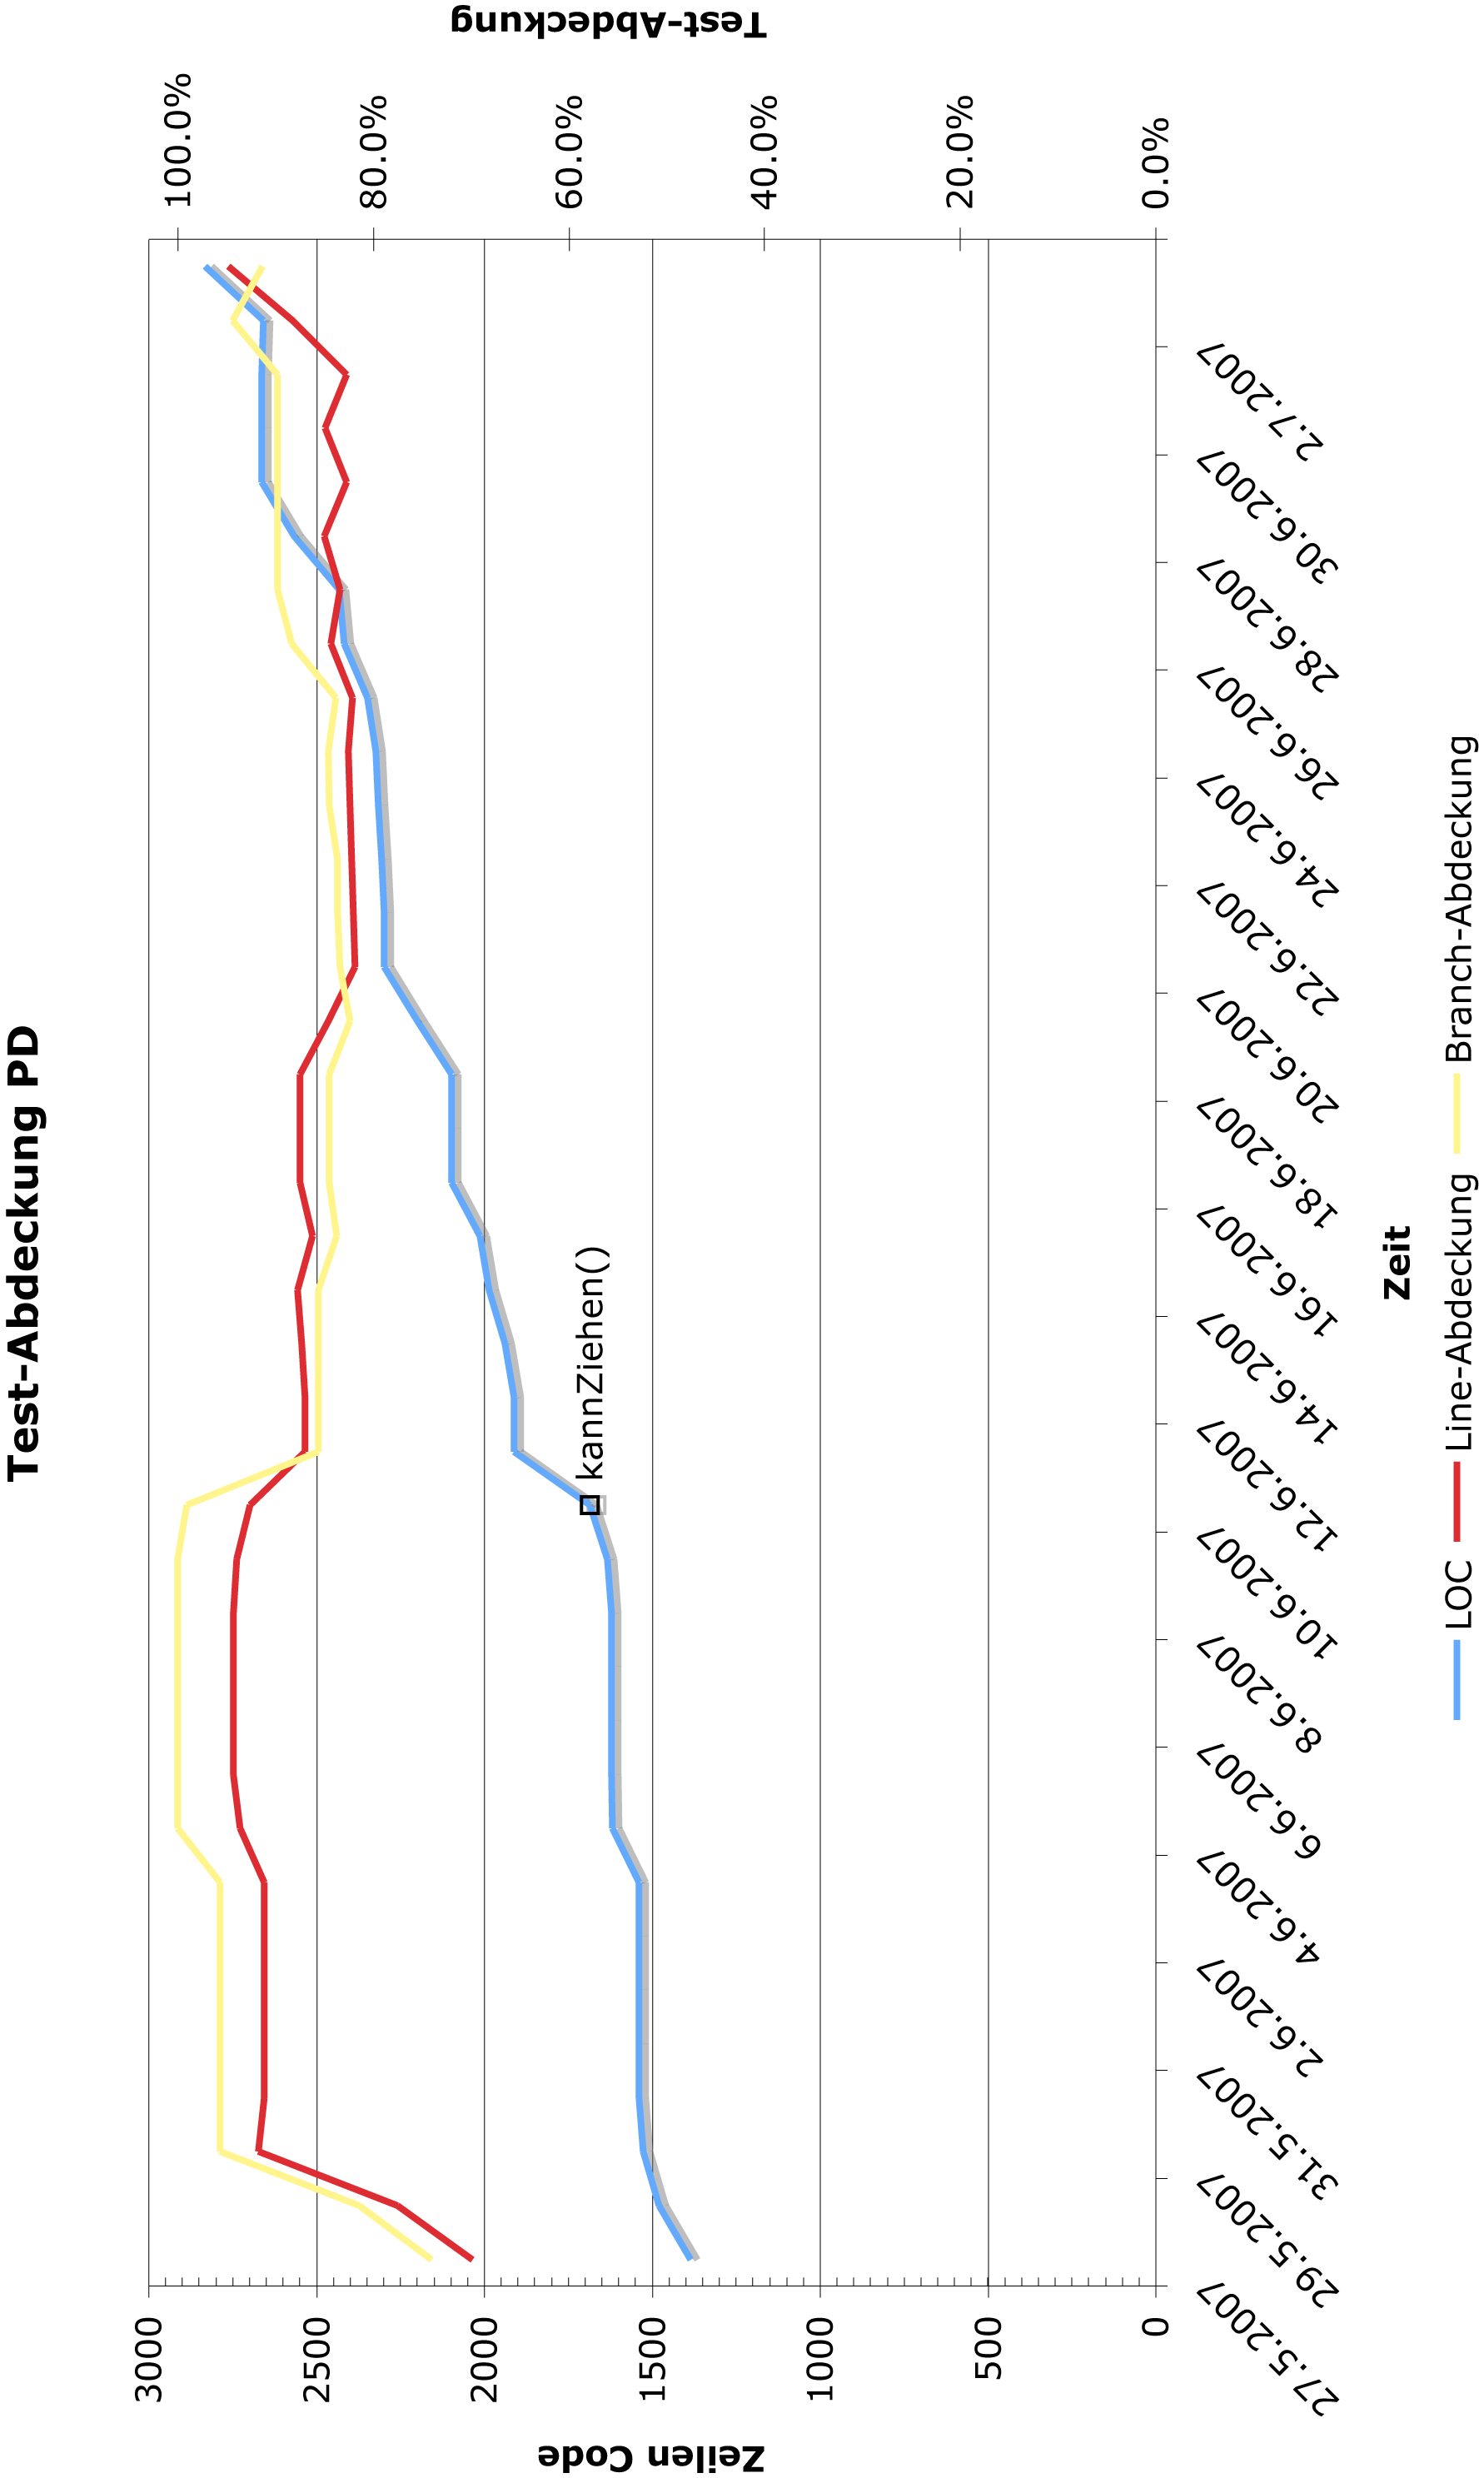
\includegraphics[width=0.8 \textwidth]{test_abdeckung_pd}
	\caption{Testabdeckung der Problem-Domain}
	\label{fig:test_abdeckung_pd}
\end{figure}

\subsection{Analyse der Anzahl von Zeilen pro Package}
Wenn man sich die Anzahl der Zeilen im Verhältnis zu den Packages anschaut, so stellt man fest, dass fundametale Packages wie die Dienstschicht oder die Problem-Domain über längere Zeit relativ konstant blieben. Andere Packages wie der Server, der Client oder das GUI wuchsen gegen Projektende markant schneller.
\begin{figure}[h]
	\centering
	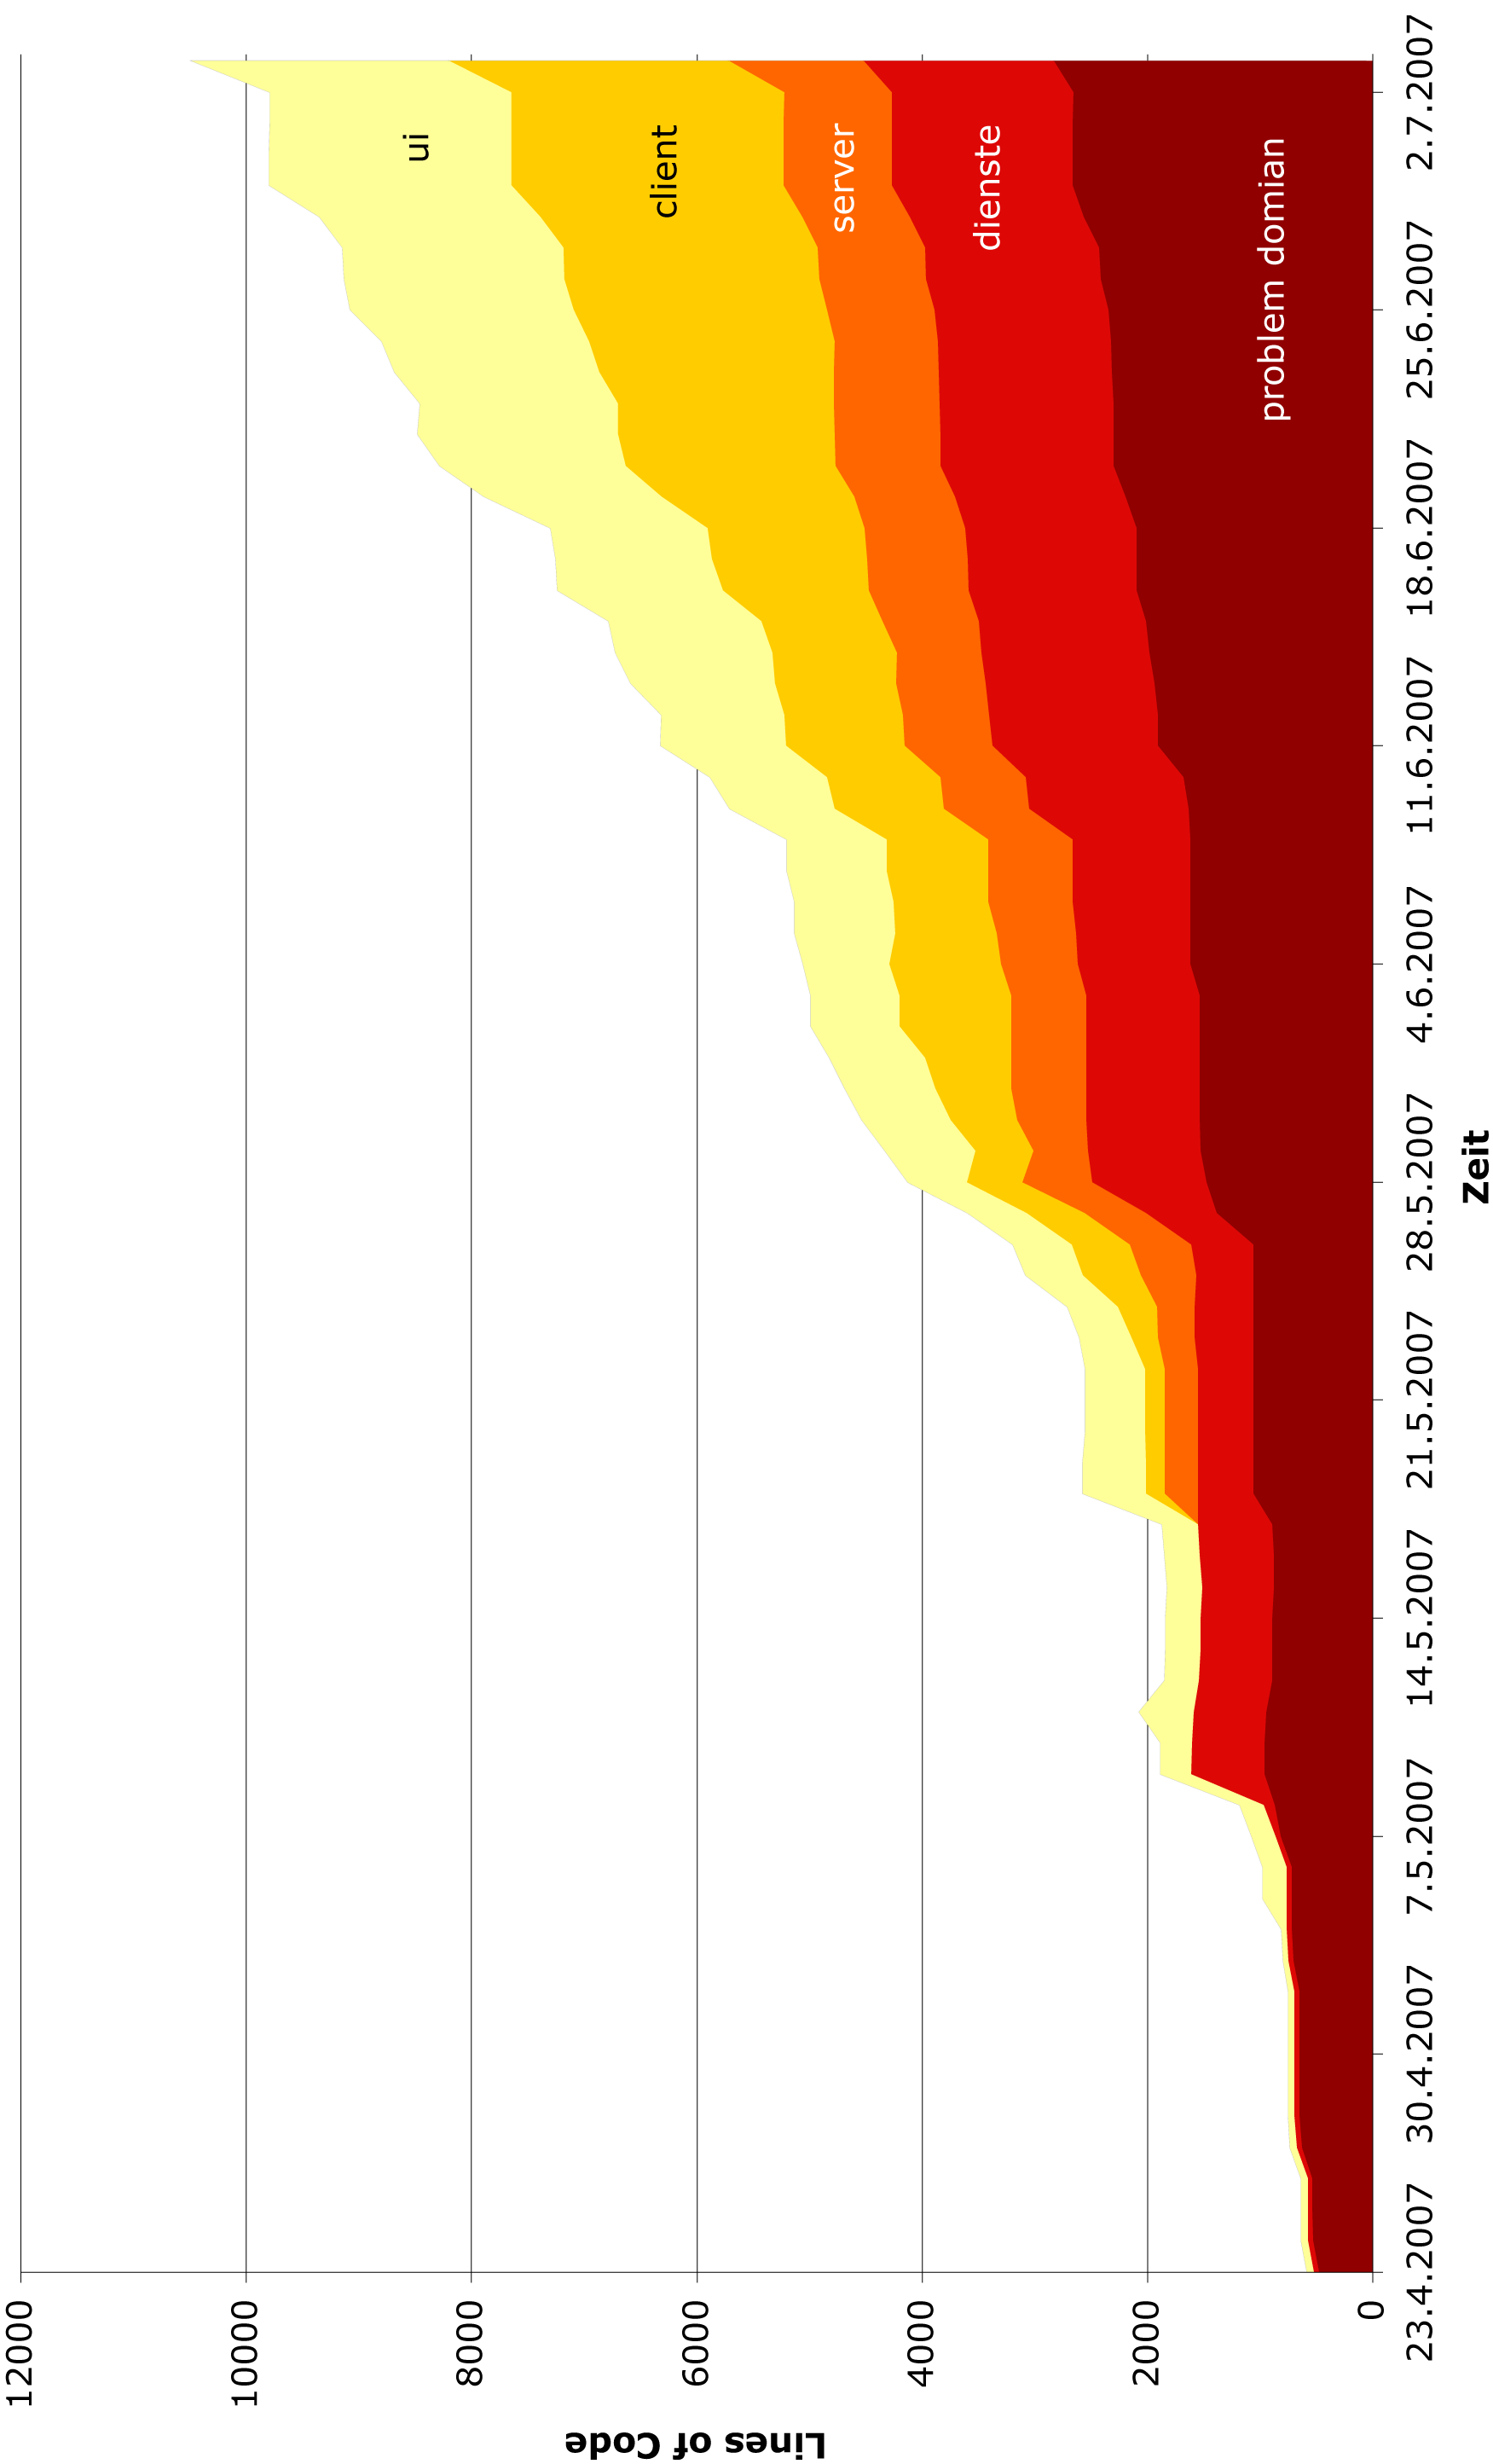
\includegraphics[width=0.8 \textwidth]{anzahl_zeilen_pro_package}
	\caption{Anzahl Zeilen Code pro Package}
	\label{fig:anzahl_zeilen_pro_package}
\end{figure}

\subsection{Aussagen zur Code-Qualität}
Mit dem Tool "<Structure 101"> waren wir in der Lage, Aussagen über die Code-Qualität zu treffen. Im Diagramm sieht man als negativen Wert "<Fette Instruktionen">. Damit sind zyklische Paketabhängkeiten, fette Methoden und Klassen gemeint.
\begin{figure}[h]
	\centering
	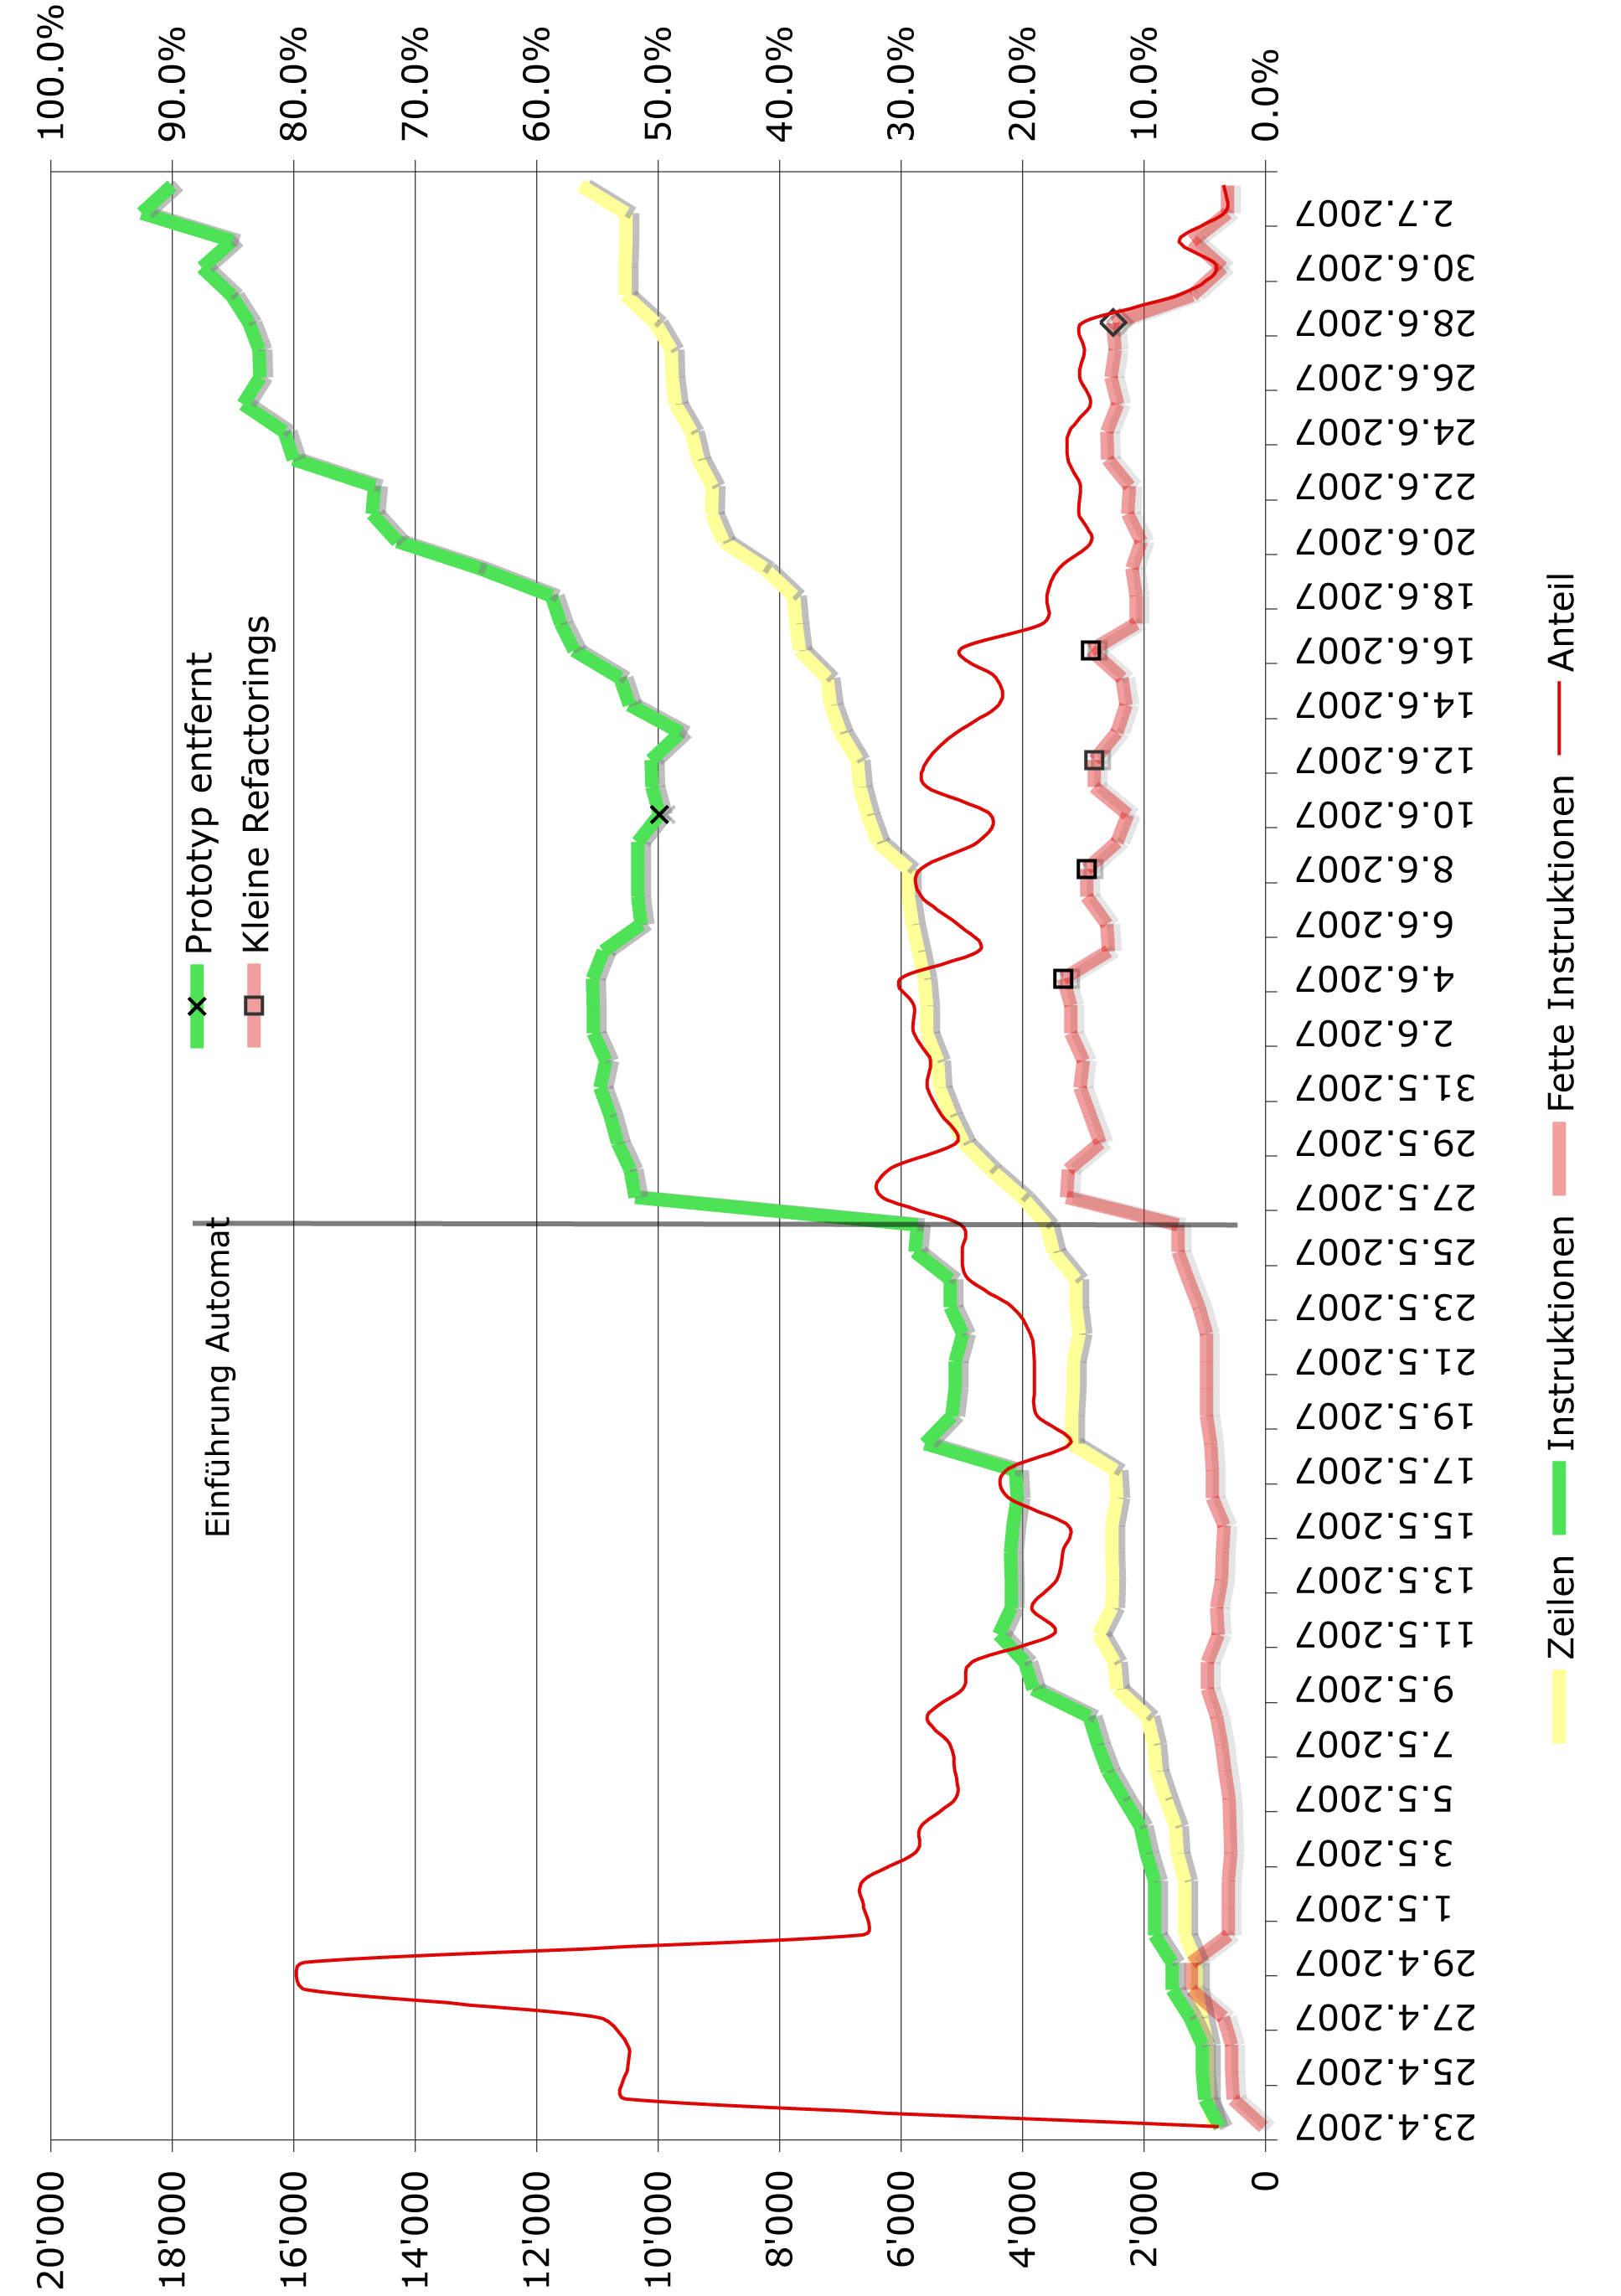
\includegraphics[width=0.8 \textwidth]{code_qualitaet}
	\caption{Aussagen zur Code-Qualität}
	\label{fig:code_qualitaet}
\end{figure}

\end{document}
